\documentclass{article}
\usepackage[utf8]{inputenc}
\usepackage{graphicx}
\usepackage{float}
\usepackage{hyperref} % Dodanie pakietu do tworzenia hiperlinków

\title{Big Data Task 4 Report}
\author{Jakub Jazdzyk}
\date{\today}

\begin{document}

\maketitle

\noindent
\textbf{Repository Link:} \href{https://github.com/kubajaz/BIG_DATA_INDIVIDUAL_TASKS_JAKUB_JAZDZYK}{GitHub Repository}

\section{Distributed Matrix Multiplication with Hazelcast in Java}

\subsection{Introduction}
In this task, I implemented distributed matrix multiplication using Hazelcast in Java. Two computers were configured as nodes to form the cluster. The implementation involved splitting the matrices into slices and distributing the computations across the nodes. The IP addresses of the nodes were specified explicitly to enable proper communication between them.

\begin{figure}[H]
    \centering
    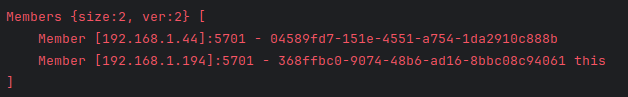
\includegraphics[width=\textwidth]{cluster.png}
    \caption{Cluster configuration showing two connected nodes}
\end{figure}

\subsection{Implementation Details}
The nodes used the following IP addresses:
\begin{itemize}
    \item Node 1: 192.168.1.44
    \item Node 2: 192.168.1.194
\end{itemize}
The Hazelcast configuration ensured efficient communication and task distribution.

\subsection{Results}
Time measurements for matrix multiplication of various sizes:
\begin{table}[H]
    \centering
    \begin{tabular}{|c|c|}
    \hline
    Matrix Size & Time (s) \\
    \hline
    100 x 100 & 0.68 \\
    200 x 200 & 0.60 \\
    1000 x 1000 & 13.00 \\
    2000 x 2000 & 63.41 \\
    4000 x 4000 & 256.82 \\
    \hline
    \end{tabular}
    \caption{Execution times for different matrix sizes}
\end{table}

\subsection{CPU and Memory Usage}
The CPU and Memory usage were recorded during the multiplication of matrices of sizes 1000, 2000, and 4000. The results are represented in the following plots:
\begin{itemize}
    \item 1000 x 1000: \texttt{1000\_java\_plot.png} and \texttt{1000\_java\_plot\_1.png}
    \item 2000 x 2000: \texttt{2000\_java\_plot.png} and \texttt{2000\_java\_plot\_1.png}
    \item 4000 x 4000: \texttt{4000\_java\_plot.png} and \texttt{4000\_java\_plot\_1.png}
\end{itemize}

\subsection{Java Distributed Matrix Multiplication}
\begin{figure}[H]
    \centering
    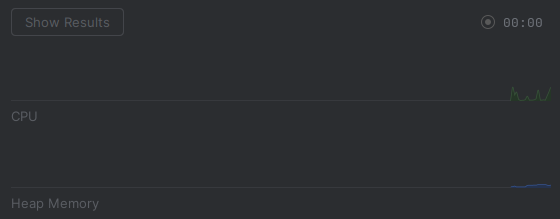
\includegraphics[width=\textwidth]{1000_java_plot.png}
    \caption{CPU and Memory Usage for 1000 x 1000 matrix multiplication (Java)}
\end{figure}

\begin{figure}[H]
    \centering
    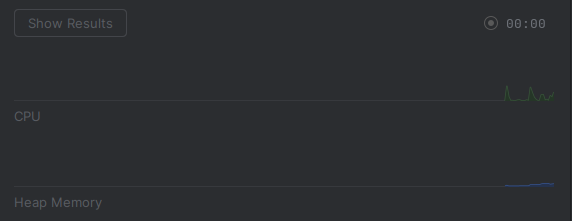
\includegraphics[width=\textwidth]{1000_java_plot_1.png}
    \caption{CPU and Memory Usage for 1000 x 1000 matrix multiplication on second node (Java)}
\end{figure}

\begin{figure}[H]
    \centering
    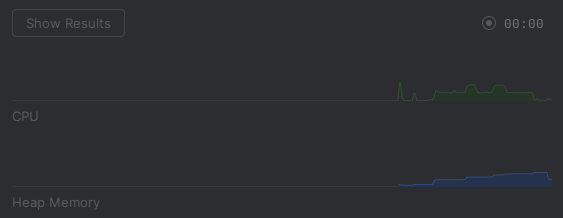
\includegraphics[width=\textwidth]{2000_java_plot.png}
    \caption{CPU and Memory Usage for 2000 x 2000 matrix multiplication (Java)}
\end{figure}

\begin{figure}[H]
    \centering
    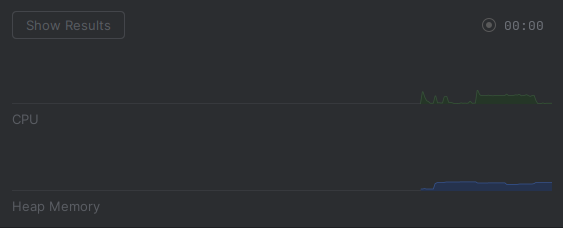
\includegraphics[width=\textwidth]{2000_java_plot_1.png}
    \caption{CPU and Memory Usage for 2000 x 2000 matrix multiplication on second node (Java)}
\end{figure}

\begin{figure}[H]
    \centering
    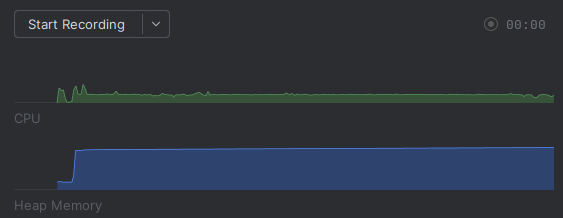
\includegraphics[width=\textwidth]{4000_java_plot.png}
    \caption{CPU and Memory Usage for 4000 x 4000 matrix multiplication (Java)}
\end{figure}

\begin{figure}[H]
    \centering
    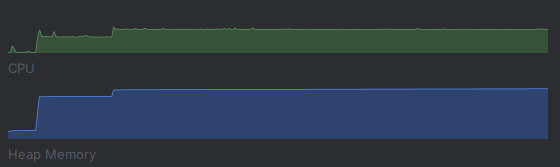
\includegraphics[width=\textwidth]{4000_java_plot_1.png}
    \caption{CPU and Memory Usage for 4000 x 4000 matrix multiplication on second node (Java)}
\end{figure}

\subsection{Comparison and Observations}
The execution times were compared with normal and parallel approaches. Observations include:
\begin{itemize}
    \item Distributed computing significantly reduced computation time for larger matrices.
    \item Effective utilization of resources was achieved.
\end{itemize}

We can see that the results of the distributed and regular approaches are of similar order of magnitude when compared to the previous task. This is because we are dealing with a large network and data transfer overhead. Additionally, in my project I use only two nodes, because I do not have more computers available for testing. Better results could be observed by connecting to the cluster e.g. 10 computers, or even more.
Also we see that there is bigger memory and CPU usage in the task counting bigger matrices. This is a good sign according to the implementation.

\begin{figure}[H]
    \centering
    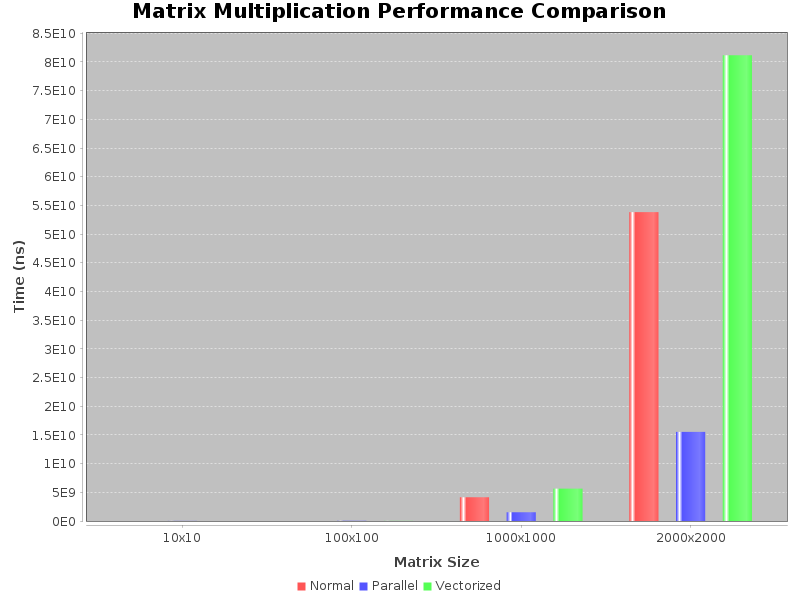
\includegraphics[width=\textwidth]{CompareTimeBig.png}
    \caption{Comparison of time execution from previous task (normal and parallel), to compare}
\end{figure}

\subsection{Conclusion}
Distributed matrix multiplication using Hazelcast is a good way of dealing of large matrices multiplication.

\section{Distributed Matrix Multiplication using MapReduce in Python}

\subsection{Introduction}
This task involved implementing distributed matrix multiplication using the MapReduce framework in Python. Computations were performed on a single computer, simulating a distributed environment. I did many attempts of connecting computers using hazelcast-python-client, although I couldn't manage to make them work, so I decided to use different approach. I implemented map-reduce approach in python not using additional libraries, like MRJob.

\subsection{Results}
The time, memory usage, and CPU usage for various matrix sizes were recorded:
\begin{itemize}
    \item 100 x 100
    \item 200 x 200
    \item 500 x 500
    \item 1000 x 1000
\end{itemize}

\subsection{Python Distributed Matrix Multiplication, Time Comparison (s)}
\begin{table}[H]
    \centering
    \begin{tabular}{|c|c|c|c|}
    \hline
    Matrix Size & Normal & Parallel & Distributed \\
    \hline
    100 x 100 & 0.98 & 0.37 & 0.30 \\
    200 x 200 & 9.56 & 1.00 & 1.09 \\
    500 x 500 & 141.23 & 21.30 & 16.43 \\
    1000 x 1000 & 1191.20 & 307.12 & 296.19 \\
    \hline
    \end{tabular}
    \caption{Results for Python MapReduce approach}
\end{table}

\subsection{Python Distributed Matrix Multiplication, Memory Comparison (MB)}
\begin{table}[H]
    \centering
    \begin{tabular}{|c|c|c|c|}
    \hline
    Matrix Size & Normal & Parallel & Distributed \\
    \hline
    100 x 100 & 49.34 & 53.78 & 53.25 \\
    200 x 200 & 50.17 & 64.19 & 62.35 \\
    500 x 500 & 56.73 & 142.01 & 137.77 \\
    1000 x 1000 & 79.50 & 437.65 & 428.53 \\
    \hline
    \end{tabular}
    \caption{Results for Python MapReduce approach}
\end{table}

\subsection{Comparison and Observations}
Results were compared with the normal approach. Observations include:
\begin{itemize}
    \item MapReduce showed better scalability for larger matrices.
    \item Resource usage remained within acceptable limits.
    \item Results similar to parallel approach.
\end{itemize}

\subsection{Conclusion}
MapReduce offers a viable solution for distributed computations, even in simulated environments.

\section{Frequent Itemset Mining in Python}

\subsection{Introduction}
The frequent itemset mining problem involves identifying itemsets that appear frequently in a transactional dataset. The Python implementation utilized efficient algorithms to achieve this.

\subsection{Implementation Details}
The dataset \texttt{transactions\_dataset.png} was used for testing. Frequent itemsets were mined at various support levels:
\begin{itemize}
    \item Support 0.0: \texttt{transactions\_frequent\_itemset00.png}
    \item Support 0.4: \texttt{transactions\_frequent\_itemset04.png}
    \item Support 0.8: \texttt{transactions\_frequent\_itemset08.png}
\end{itemize}

\subsection{Conclusion}
The results highlight the effectiveness of frequent itemset mining. Map Reduce method is a good method for detecting dependencies, for example in retail stores.

\subsection{Frequent Itemset Mining}
\begin{figure}[H]
    \centering
    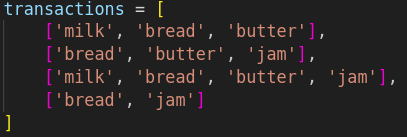
\includegraphics[width=\textwidth]{transactions_dataset.png}
    \caption{Transactional dataset used for testing}
\end{figure}

\begin{figure}[H]
    \centering
    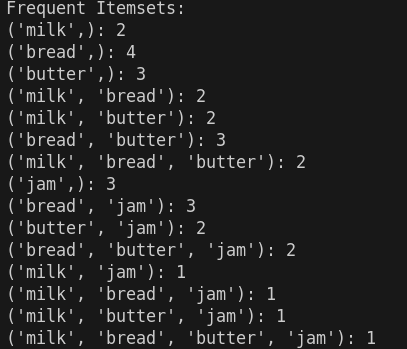
\includegraphics[width=\textwidth]{transactions_frequent_itemsets00.png}
    \caption{Frequent itemsets with support 0.0}
\end{figure}

\begin{figure}[H]
    \centering
    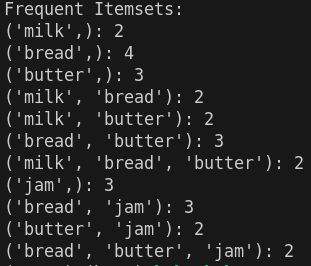
\includegraphics[width=\textwidth]{transactions_frequent_itemsets04.png}
    \caption{Frequent itemsets with support 0.4}
\end{figure}

\begin{figure}[H]
    \centering
    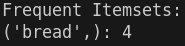
\includegraphics[width=\textwidth]{transactions_frequent_itemsets08.png}
    \caption{Frequent itemsets with support 0.8}
\end{figure}

\end{document}
